\section{Thermal Hydraulics}
\label{sec:thermalHydraulics}

\begin{frame}{Assembly Geometry}
  \begin{figure}
    \centering
    \subfloat{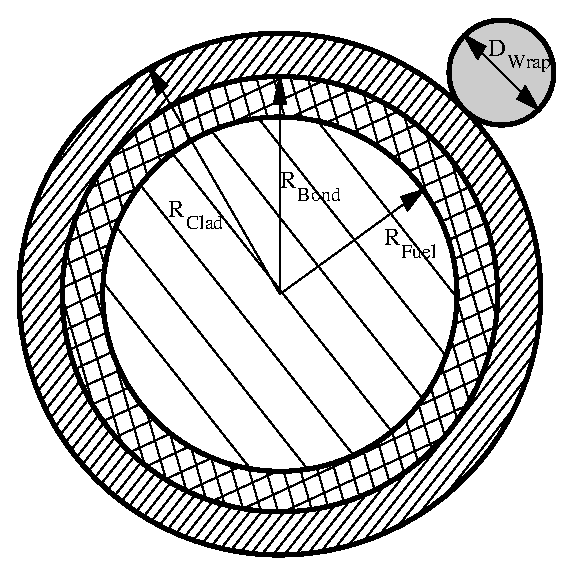
\includegraphics[width=0.4\textwidth]{pin_model}}
    \hspace{0.2in}
    \subfloat{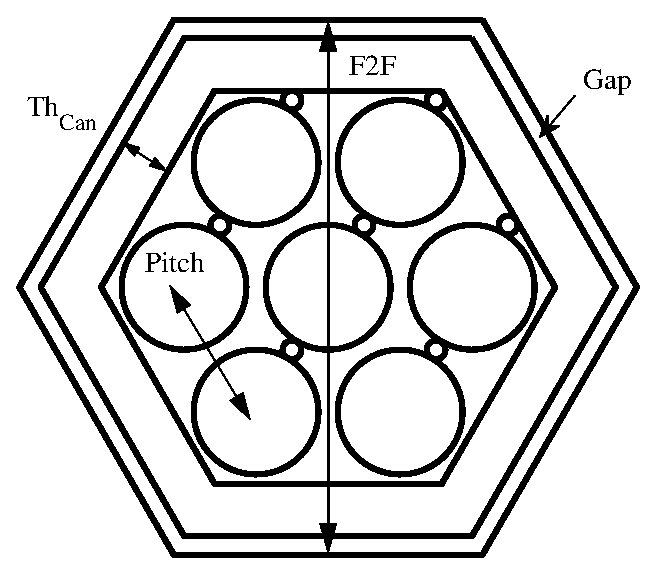
\includegraphics[width=0.4\textwidth]{hex_can}}
    \label{fig:assy_geometry}
  \end{figure}
\end{frame}

\begin{frame}{Material Properties}
  \begin{itemize}
    \item Functional sodium properties \cite{sodiumProp}.
    \item Clad and bond thermal conductivity assumed constant \cite{ht9Prop}.
    \item Fuel thermal conductivity assumed a function of temperature
      \cite{fuelProp}.
  \end{itemize}
  \begin{figure}
    \centering
    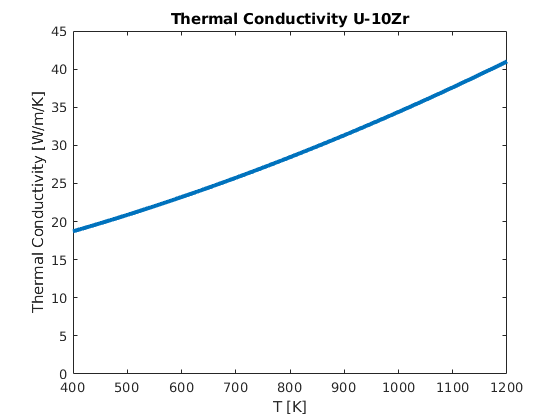
\includegraphics[width=0.7\textwidth]{kfuel_plot}
    %\caption{Variable Thermal Conductivity in Fuel.}
    \label{fig:kfuel_plot}
  \end{figure}
\end{frame}

\begin{frame}{Axial Convection Geometric Model}
  \begin{columns}
    \begin{column}{0.5\textwidth}
      \begin{figure}
        \centering
        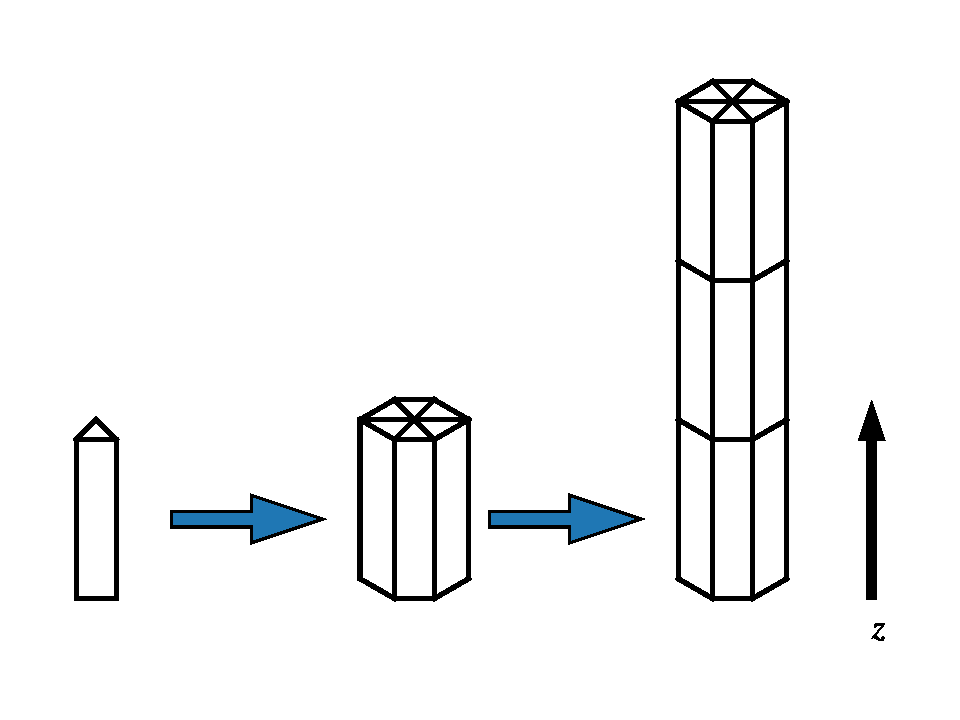
\includegraphics[width=\textwidth]{chunk_description}
        \caption{Progression of Element (left), to Chunk (center), to Channel
          (right).}
        \label{fig:chunk_description}
      \end{figure}
    \end{column}
    \begin{column}{0.5\textwidth}
      \begin{figure}
        \centering
        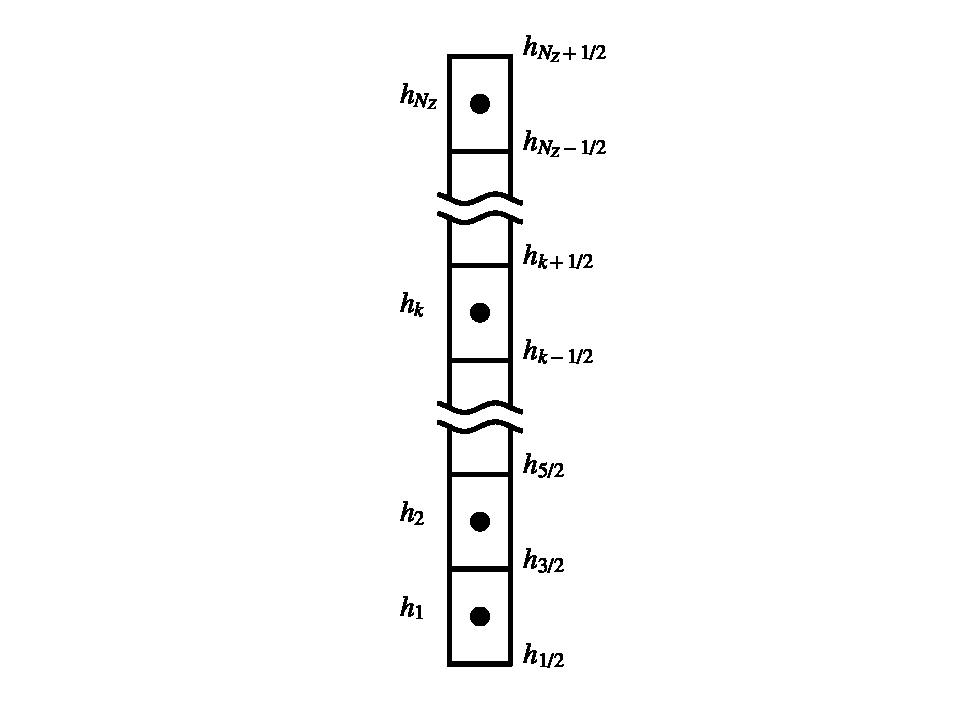
\includegraphics[width=0.35\textwidth]{axial_model}
        %\caption{One-Dimensional Axial Heat Convection Model Description.}
        \caption{Nodalization for channel $i$.}
        \label{fig:axial_model}
      \end{figure}
    \end{column}
  \end{columns}
\end{frame}

\begin{frame}{Channel Enthalpy}
  Steady-state coolant enthalpy within the channel is given by an energy
  balance.
  \begin{equation}
    h_{i,k+1/2} = h_{in} + \frac{1}{\mdot_i} \sum_{k'=1}^{k} q_{i,k'}
  \end{equation}
  Use a first-order approximation to estimate the chunk-average enthalpy.
  \begin{equation}
    h_{i,k} = \half (h_{i,k-1/2}+h_{i,k+1/2})
  \end{equation}
  $T_{\infty,i,k}$ is then given by a state relationship \cite{sodiumProp}.
  \begin{equation}
    T_{\infty,i,k} = T(h_{i,k})
  \end{equation}
\end{frame}

\begin{frame}{Radial Conduction Geometric Model}
  \begin{figure}
    \centering
    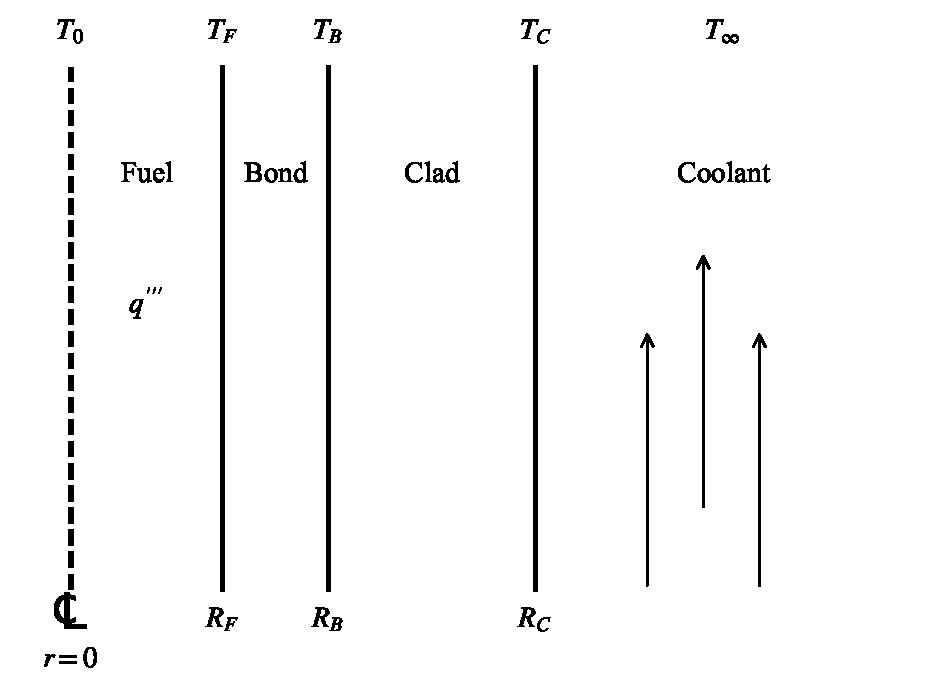
\includegraphics[width=0.7\textwidth]{radial_model}
    \caption{Geometry Description of Radial Heat Conduction Model (not to
      scale).}
    \label{fig:radial_model}
  \end{figure}
\end{frame}

\begin{frame}{Clad Surface Temperature -- Subbotin-Ushakov}
  Using Newton's Law of Cooling.
  \begin{align}
    q''_{clad} &= H_c (T_C - T_{\infty}) %\\
    %q''_{clad} &= q'''_{i,k} \frac{R_F^2}{2 R_C}
  \end{align}
  $H_c$ is given by the Subbotin-Ushakov correlation \cite{subbotinUshakov}
  which relates the Nusselt and P\'eclet numbers for ${1 < Pe < 4,000}$ and 
  ${ 1.2 \le S/D \le 2.0 }$.
  \begin{align}
    Pe &= Re \, Pr \\
    \label{eq:subbotinUshakov}
    Nu &= 7.55 \frac{S}{D} - 20 \left(\frac{S}{D}\right)^{-13} + 
      \frac{3.67}{90\left(\frac{S}{D}\right)^{2}}
      Pe^{\left(0.56 + 0.19 \frac{S}{D}\right)} \\
    H_c &= \frac{N\!u \, k}{D_e} %\\
  \end{align}
  Then, the clad surface temperature, $T_C$ follows.
\end{frame}

\begin{frame}{Fuel Centerline Temperature}
  Define a conductivity integral.
  \begin{equation}
    \label{eq:conductivity_integral}
    K_F(T) = \int_0^T k_F(T') \; dT'
  \end{equation}
  The value of the conductivity integral is given by the heat conduction
  equation.
  \begin{equation}
    \label{eq:tcl_conductivity_integral}
    K_F(T_0) = K_F(T_F) + \frac{q'''_{i,k}}{4} R_F^2
  \end{equation}
  Then, a bisection method search is used to calculate $T_0$ given a functional
  form of $K_F(T)$.
\end{frame}

\begin{frame}{Average Material Temperatures}
  Average temperatures in the clad and bond are calculated analytically.
  \begin{align}
    \label{eq:tc_bar}
    \overline{T_C} &= T_B - \frac{q'''}{4 k_C} R_F^2 \left(
      \frac{2 \, R_C^2 \ln\left(\frac{R_C}{R_B}\right)}
      {R_C^2 - R_B^2}  - 1\right) \\
    \label{eq:tb_bar}
    \overline{T_B} &= T_F - \frac{q'''_{i,k}}{4 k_B} \, R_F^2 \, \left(
      \frac{R_F^2 - R_B^2 + 2\,R_B^2 \ln\left(\frac{R_B}{R_F}\right)}
      {R_B^2-R_F^2}\right)
  \end{align}
\end{frame}

\begin{frame}{Average Fuel Temperature}
  Calculate an effective thermal conductivity in the fuel.
  \begin{equation}
    \label{eq:kfuel_constant}
    \overline{k_F} = \frac{q'''_{i,k} \, R_F^2}{4(T_0-T_F)}
  \end{equation}
  Assume thermal conductivity is constant $\overline{k_F}$.\\
  Calculate an analytic value for the average fuel temperature.
  \begin{equation}
    \label{eq:tf_bar}
    \overline{T_F} = T_0 - \frac{q'''_{i,k}}{8 \overline{k_F}} R_F^2
  \end{equation}
  $\overline{T_F}$ is used to calculate fuel cross sections. \\
  Due to self-shielding, an effective fuel temperature would weight the surface 
  temperature more.
\end{frame}

\begin{frame}{Radial Temperatures for Typical Fuel Rod}
  \begin{figure}
    \centering
    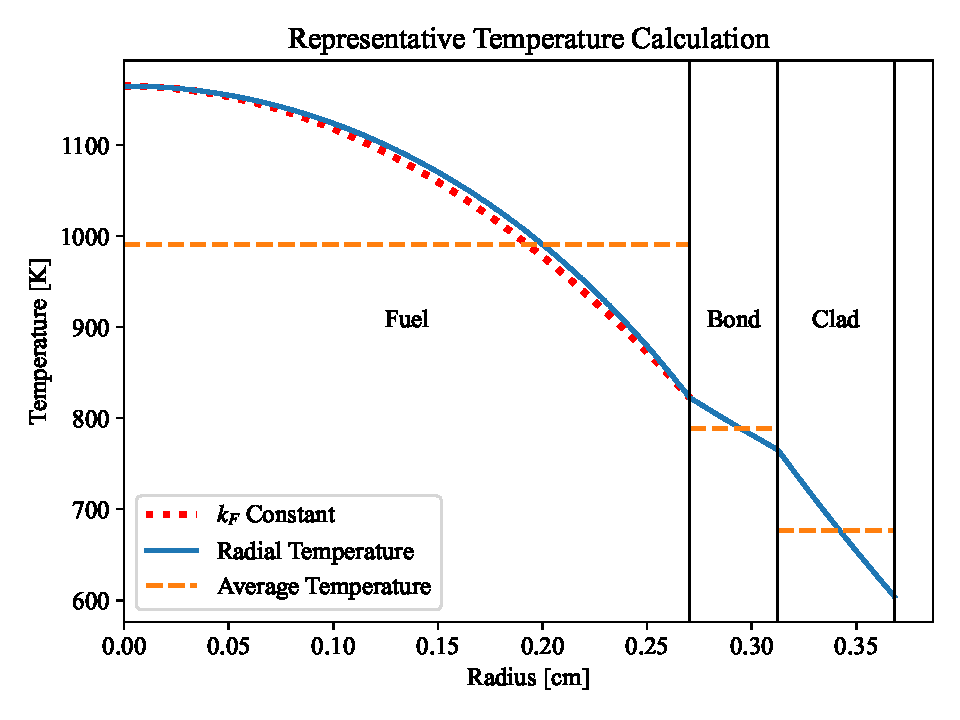
\includegraphics[width=0.7\textwidth]{radial_temp_plot}
    %\caption{Radial Temperatures for Typical Fuel Rod.}
    \label{fig:radial_temp_plot}
  \end{figure}
  \begin{block}{}
    \centering
    Difference less than 15 \units{K}.
  \end{block}
\end{frame}

%\begin{frame}{Cross Section Treatment}
%  \begin{itemize}
%    \item Coolant. 
%      \begin{itemize}
%        \item Number density and microscopic cross sections are functionalized.
%        \item Linear interpolation for microscopic cross sections.
%      \end{itemize}
%      \begin{align}
%        N_{Na}(T) &= \frac{\rho_{Na}(T) \, N_A}{M_{Na}}\\
%        \label{eq:xs_cool}
%        \Sigma_{x,i,k,g} &= N_{Na}(T_{\infty,i,k}) 
%          \left( \frac{T_{\infty,i,k} - T_{n}}{T_{n+1}-T_{n}} 
%          (\sigma_{x,Na,g,n+1} - \sigma_{x,Na,g,n})  + \sigma_{x,Na,g,n}\right)
%      \end{align}
%    \vspace{-\baselineskip}
%    \item Clad. 
%      \begin{itemize}
%        \item Linear interpolation for macroscopic cross sections.
%      \end{itemize}
%      \begin{equation}
%        \label{eq:xs_linear_interpolation}
%        \Sigma_{x,i,k,g} = 
%          \frac{\overline{T_{C,i,k}} - T_{n}}{T_{n+1}-T_{n}} 
%          (\Sigma_{x,g,n+1} - \Sigma_{x,g,n})  + \Sigma_{x,g,n}
%      \end{equation}
%    \vspace{-2\baselineskip}
%    \item Bond.
%      \begin{itemize}
%        \item Assumed to have the same macroscopic cross section as coolant.
%        \item Consistent with homogenization approximation.
%      \end{itemize}
%    \item Fuel.
%      \begin{itemize}
%        \item Square-root interpolation for macrscopic cross sections due to 
%          Doppler effect. 
%      \end{itemize}
%      \begin{equation}
%        \Sigma_{x,i,k,g} = 
%          \frac{\sqrt{\overline{T_{F,i,k}}} - \sqrt{T_{n}}}
%          {\sqrt{T_{n+1}}-\sqrt{T_{n}}}
%          (\Sigma_{x,g,n+1} - \Sigma_{x,g,n})  + \Sigma_{x,g,n}
%      \end{equation}
%  \end{itemize}
%\end{frame}

\begin{frame}{Cross Section Treatment -- Coolant \& Bond}
  \begin{itemize}
    \item Number density and microscopic cross sections are functionalized 
      and updated based on $T_{\infty,i,k}$.
    \item Linear interpolation for microscopic cross sections.
  \end{itemize}

  Number density functionalization.
  \begin{align}
    \label{eq:number_density_sodium}
    M_{Na} &= 22.989769 \units{$\frac{\text{gram}}{\text{mol}}$} \\
    N_{Na}(T) &= \frac{\rho_{Na}(T) \, N_A}{M_{Na}}
  \end{align}

  Microscopic cross section functionalization for ${T_{n} < T_{\infty,i,k} <
  T_{n+1}}$.
  \begin{equation}
    \label{eq:xs_cool}
    \Sigma_{x,i,k,g} = N_{Na}(T_{\infty,i,k}) 
      \left( \frac{T_{\infty,i,k} - T_{n}}{T_{n+1}-T_{n}} 
      (\sigma_{x,Na,g,n+1} - \sigma_{x,Na,g,n})  + \sigma_{x,Na,g,n}\right)
  \end{equation}

  Bond is assumed to have the same macroscopic cross section as coolant.\\
  Consistent with homogenization approximation.
\end{frame}

\begin{frame}{Cross Section Treatment -- Clad}
  \begin{itemize}
    \item Macroscopic cross section updated based on $\overline{T_{C,i,k}}$.
    \item Linear interpolation.
  \end{itemize}

  Macroscopic cross section functionalization for ${T_n < \overline{T_{C,i,k}} <
  T_{n+1}}$.
  \begin{equation}
    \label{eq:xs_linear_interpolation}
    \Sigma_{x,i,k,g} = 
      \frac{\overline{T_{C,i,k}} - T_{n}}{T_{n+1}-T_{n}} 
      (\Sigma_{x,g,n+1} - \Sigma_{x,g,n})  + \Sigma_{x,g,n}
  \end{equation}
\end{frame}

\begin{frame}{Cross section Treatment -- Fuel}
  \begin{itemize}
    \item Macroscopic cross section update based on $\overline{T_{F,i,k}}$.
    \item Square-root interpolation due to Doppler effect.
  \end{itemize}

  Macroscopic cross section functionalization for ${T_n < \overline{T_{F,i,k}} <
  T_{n+1}}$.
  \begin{equation}
    \Sigma_{x,i,k,g} = 
      \frac{\sqrt{\overline{T_{F,i,k}}} - \sqrt{T_{n}}}
      {\sqrt{T_{n+1}}-\sqrt{T_{n}}}
      (\Sigma_{x,g,n+1} - \Sigma_{x,g,n})  + \Sigma_{x,g,n}
  \end{equation}
\end{frame}
